\documentclass[10pt,a4paper,ragged2e,withhyper]{altacv}

% -----------------------
% PACKAGES
% -----------------------
\usepackage[utf8]{inputenc}
\usepackage[T1]{fontenc}
\usepackage{paracol} % Needed for two-column layout
\usepackage{graphicx}
\usepackage{svg}
\svgpath{{icons/}}
\usepackage{fontawesome5}
\usepackage{hyperref}
\usepackage{pgfplots}
\usepackage{tikz}
\usepackage{enumitem}
\usepackage{xcolor}
\usepackage{geometry}
\usepackage{ragged2e, microtype} % ensure this is in the preamble
\usetikzlibrary{shapes, shadows}

% -----------------------
% MODERN DEVELOPER FONTS
% -----------------------
% Use monospace font for developer aesthetic
\usepackage{lmodern}
\renewcommand{\familydefault}{\ttdefault} % Use typewriter font
\usepackage[scaled=0.85]{beramono} % Modern monospace font

% -----------------------
% DOCKER-INSPIRED COLOR PALETTE
% -----------------------
\definecolor{DockerBlue}{HTML}{2496ED}      % Docker Primary Blue
\definecolor{DockerDark}{HTML}{24292F}      % GitHub Dark
\definecolor{DockerLight}{HTML}{F6F8FA}     % GitHub Light Background
\definecolor{DockerGray}{HTML}{6A737D}      % GitHub Gray Text
\definecolor{DockerSuccess}{HTML}{28A745}   % Success Green
\definecolor{DockerWarning}{HTML}{FFC107}   % Warning Yellow
\definecolor{DockerDanger}{HTML}{DC3545}    % Error Red
\definecolor{DockerPurple}{HTML}{6F42C1}    % Purple accent
\definecolor{DockerBorder}{HTML}{E1E4E8}    % Light border

% Modern color assignments
\colorlet{heading}{DockerBlue}
\colorlet{accent}{DockerBlue}
\colorlet{emphasis}{DockerDark}
\colorlet{body}{DockerGray}
\colorlet{lightbg}{DockerLight}
\colorlet{border}{DockerBorder}

% -----------------------
% MODERN 2024 LAYOUT
% -----------------------
\geometry{margin=0.5cm} % 1cm margins as requested
\usetikzlibrary{positioning,shapes.geometric,arrows.meta,shadows,decorations.pathreplacing}
\usepackage{tcolorbox}
\tcbuselibrary{skins}
\usepackage{tikz}

% Card with tiny light border, rounded corners
\tcbset{
  vercelcard/.style={
    enhanced,
    boxrule=0.4pt,
    colback=white,
    colframe=DockerBorder,
    arc=6pt,
    outer arc=6pt,
    top=14pt,
    bottom=14pt,
    left=18pt,
    right=18pt,
    boxsep=0pt
  }
}

% Timeline card with light border
\tcbset{
  timelinecard/.style={
    enhanced,
    boxrule=0.5pt,
    colback=white,
    colframe=DockerBorder,
    arc=6pt,
    top=12pt,
    bottom=12pt,
    left=16pt,
    right=16pt
  }
}

% Modern skill icon with SVG support (SVG files in icons/)
% Use center baseline and zero inner sep to avoid vertical misalignment across SVGs
\newcommand{\skillicon}[2]{%
  \tikz[baseline=(icon.center)]{
    \node[circle, fill=#1!8, draw=#1!20, minimum size=22pt, inner sep=0pt] (icon) {\includesvg[width=12pt,height=12pt]{#2}};
  }%
}

% Fallback text icon for missing SVGs
\newcommand{\textskillicon}[2]{%
  \tikz[baseline=(icon.base)]{
    \node[circle, fill=#1!8, draw=#1!20, minimum size=22pt, font=\tiny\ttfamily] (icon) {#2};
  }%
}

% Timeline node command
\newcommand{\timelinenode}[1]{%
  \tikz[baseline=(node.base)]{
    \node[circle, fill=#1, minimum size=12pt, inner sep=0pt] (node) {};
  }%
}

% Timeline layout paddings and fixed text width
\newlength{\timelineLeftPad}
\newlength{\timelineRightPad}
\newcommand{\timelineTextWidth}{\dimexpr\linewidth-\timelineLeftPad-\timelineRightPad\relax}
\tikzset{timelineTextNode/.style={text width=\timelineTextWidth, inner sep=0pt, align=justify}}


% Horizontal percentage skill bar
\newcommand{\skillbar}[2]\par\vspace{2pt}%
  \begin{tikzpicture}[x=\linewidth,y=1cm]
    \fill[DockerBorder] (0,0) rectangle (1,0.12);
    \pgfmathsetmacro{\p}{#2/100}
    \fill[DockerBlue] (0,0) rectangle (\p,0.12);
  \end{tikzpicture}\vspace{4pt}
}

% Project item macro (uniform format)
\newcommand{\projectitem}[3]{%
  \textbf{#1}\\
  \textcolor{body}{#2}\\[4pt]
  % Only show GitHub tag if #3 is not empty
  \if\relax\detokenize{#3}\relax
    % do nothing
  \else
    \cvtag{\faGithub\ \href{https://github.com/#3}{#3}}\\
  \fi
}

% -----------------------
% PERSONAL INFO
% -----------------------
\name{Marcos Oriol Pagonabarraga}
\tagline{Neuroengineer - Software Engineer}
\photoL{3cm}{photo.png} % ← Add your photo.png in same folder or comment this line

\personalinfo{
  \email{marcos.oriol.p@gmail.com}
  \phone{+34 626 027 986}
  \github{MarcosOriolPago}
  \linkedin{marcos-oriol-pagonabarraga-a9a590143}
  \homepage{marcos.oriol-tech-com}
}

% -----------------------
% DOCUMENT BODY
% -----------------------
\begin{document}
\noindent
\begin{tikzpicture}[remember picture,overlay]
  % Background gradient
  \fill[left color=DockerBlue, right color=DockerPurple]
    (current page.north west) rectangle ([yshift=-6.2cm]current page.north east);

  % Header content
  \node[anchor=north west, inner sep=0pt] at (current page.north west) {
    \begin{minipage}[c][6.2cm][c]{\paperwidth}
      \hspace*{1cm}%
      % Photo
      \begin{minipage}[c]{0.22\paperwidth}
        \centering
        \tikz{\path[fill overzoom image={photo.png}] circle[radius=2cm];}
      \end{minipage}%
      \hspace{0.3cm}%
      % Text content
      \begin{minipage}[c]{0.60\paperwidth}
        {\color{white}{\Huge\bfseries Marcos Oriol Pagonabarraga}}\\[4pt]
        {\color{white!90}{\Large Neuroengineer \& Software Engineer}}\\[6pt]
        {\small\color{white!92}{%
          \faAt\ \href{mailto:marcos.oriol.p@gmail.com}{marcos.oriol.p@gmail.com}\quad
          \faPhone\ \href{tel:+34626027986}{+34\,626\,027\,986}\quad
          \faGithub\ \href{https://github.com/MarcosOriolPago}{github.com/MarcosOriolPago}\quad
          \faLinkedin\ \href{https://www.linkedin.com/in/marcos-oriol-pagonabarraga-a9a590143/}{linkedin.com/in/marcos-oriol-pagonabarraga}\quad
          \faGlobe\ \href{https://marcos.oriol-tech.com}{marcos.oriol-tech.com}}}\\[6pt]

        % About box floating
        \tikz[baseline]{
          \node[
            draw=white!80,
            thick,
            dashed,
            rounded corners=8pt,
            inner sep=10pt,
            text width=0.95\linewidth
          ] {
            \textbf{\color{white!92}\begin{tcolorbox}[vercelcard]
\textcolor{DockerBlue}{\large\textbf{About}}

\vspace{8pt}

I am a restless individual with a strong interest in \textbf{neuroscience}. I am eager to 
keep growing and developing myself by diving into \textbf{new research} and \textbf{connecting with others} 
who share my passion.

\end{tcolorbox}}
          };
        }
      \end{minipage}
    \end{minipage}
  };
\end{tikzpicture}

% Reserve space below the overlay header (optimize vertical space)
\vspace*{5.4cm}

% About content integrated into header

% Two-column layout for the rest
\columnratio{0.58}
\begin{paracol}{2}

% LEFT COLUMN -----------------------
\begin{tcolorbox}[vercelcard]
\textcolor{DockerBlue}{\large\textbf{Career History}}

\vspace{8pt}

% Vertical timeline with dots on the left, constrained to column width
\begin{tikzpicture}[x=1cm,y=1cm]
  % vertical line within box (extended for added spacing)
  \draw[DockerBorder, line width=0.8pt] (0,0) -- (0,-12.2);

  % Entry 1 (top)
  \fill[DockerPurple] (0,0) circle (3pt);
  % Title aligned with dot
  \node[anchor=west] at (0.45,0) {\textcolor{DockerPurple}{\bfseries AI - ML Engineer}};
  % Company
  \node[anchor=west,text=emphasis] at (0.45,-0.50) {IDNEO Technologies Inc.};
  % Place
  \node[anchor=west,text=body] at (0.45,-1.00) {\small Barcelona, Spain (2024 -- present)};
  % Description (wrapped)
  \node[anchor=west,align=left,text width=\dimexpr\linewidth-1.3cm\relax] at (0.45,-2.30) 
  {Development of AI Models for embedded systems in the automotive industry, including data collection, model training, and deployment.};
  % Icons
  \node[anchor=west] at (0.45,-3.90) {\skillicon{DockerWarning}{python-original}\hspace{3pt}\skillicon{DockerBlue}{docker-original}\hspace{3pt}\skillicon{DockerDanger}{tensorflow-original}\hspace{3pt}\skillicon{DockerPurple}{pytorch-original}};

  %%%%%%%%%%%%%%%%%%%%%%%%%%%%
  % Entry 2 base y
  \def\ybase{-5}
  \fill[DockerPurple] (0,\ybase) circle (3pt);
  % Title
  \node[anchor=west] at (0.45,\ybase) {\textcolor{DockerPurple}{\bfseries Software Engineer Collaboration}};
  % Company
  \node[anchor=west,text=emphasis] at (0.45,\ybase-0.50) {PRBB - Hospital del Mar};
  % Place
  \node[anchor=west,text=body] at (0.45,\ybase-1.00) {\small Barcelona, Spain (2024 - 2025)};
  % Description
  \node[anchor=west,align=left,text width=\dimexpr\linewidth-1.3cm\relax] at (0.45,\ybase-1.9) 
  {Use of focused ultrasound (FUS) for spinal cord neuronal stimulation.};
  % Icons
  \node[anchor=west] at (0.45,\ybase-3.1) {\skillicon{DockerSuccess}{react-original}\hspace{3pt}\skillicon{DockerWarning}{python-original}\hspace{3pt}\skillicon{DockerPurple}{postgresql-original}};

  %%%%%%%%%%%%%%%%%%%%%%%%%%%%
  % Entry 3 base y
  \def\ybase{-9.1}
  \fill[DockerPurple] (0,\ybase) circle (3pt);
  % Title
  \node[anchor=west] at (0.45,\ybase) {\textcolor{DockerPurple}{\bfseries Neuroengineering Research Intern}};
  % Company
  \node[anchor=west,text=emphasis] at (0.45,\ybase-0.50) {i3S};
  % Place
  \node[anchor=west,text=body] at (0.45,\ybase-1.00) {\small Porto, Portugal (feb 2024 - jun 2024)};
  % Description
  \node[anchor=west,align=left,text width=\dimexpr\linewidth-1.3cm\relax] at (0.45,\ybase-2.50) 
  {Development of neuron models for detection of memory associated pattern in the hippocampus of mice. The neuron model was then mapped to neuromorphic hardware.};
  % Icons
  \node[anchor=west] at (0.45,\ybase-4.3) {\skillicon{DockerSuccess}{react-original}\hspace{3pt}\skillicon{DockerWarning}{python-original}\hspace{3pt}\skillicon{DockerPurple}{postgresql-original}};
\end{tikzpicture}

\end{tcolorbox}


\vspace{2pt}

\begin{tcolorbox}[
    vercelcard,
    sidebyside,
    righthand width=0.42\linewidth,
    sidebyside gap=16pt,
    sidebyside align=top  % <-- this makes both columns top-aligned
]
\textcolor{DockerBlue}{\large\textbf{Capabilities}}\\[6pt]

% LEFT: Technologies (icons)
\textcolor{emphasis}{\textbf{Technologies}} \\
\vspace{6pt}
\textbf{Frontend}\\
\vspace{6pt}
\skillicon{DockerBlue}{react-original}
\skillicon{DockerSuccess}{typescript-original}
\skillicon{DockerSuccess}{javascript-original}
\skillicon{DockerPurple}{php-original}\\[8pt]
\textbf{Backend}\\
\vspace{6pt}
\skillicon{DockerWarning}{python-original}
\skillicon{DockerPurple}{postgresql-original}\\[8pt]
\textbf{AI / ML}\\
\vspace{6pt}
\skillicon{DockerDanger}{tensorflow-original}
\skillicon{DockerPurple}{pytorch-original}
\skillicon{DockerBlue}{matlab-original}\\[8pt]
\textbf{DevOps \& Tools}\\
\vspace{6pt}
\skillicon{DockerBlue}{docker-original}
\skillicon{emphasis}{linux-original}
\skillicon{DockerGray}{github-original}
\skillicon{DockerGray}{googlecloud-original}

\tcblower
% RIGHT: Skills radar + soft skills + languages
\textcolor{emphasis}{\textbf{Skills}} \\
\begin{center}
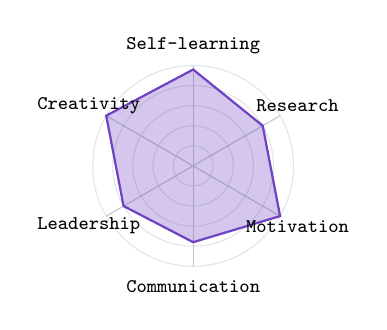
\begin{tikzpicture}[scale=0.51]
  % Draw concentric circles
  \foreach \r in {0.5,1,1.5,2,2.5} {\draw[DockerBorder, thin] (0,0) circle (\r cm);}  

  % Axes: Self-learning, Research, Motivation, Communication, Leadership, Creativity
  \draw[DockerGray!40] (0,0) -- (90:2.5cm);   % Self-learning
  \draw[DockerGray!40] (0,0) -- (30:2.5cm);   % Research
  \draw[DockerGray!40] (0,0) -- (-30:2.5cm);  % Motivation
  \draw[DockerGray!40] (0,0) -- (-90:2.5cm);  % Communication
  \draw[DockerGray!40] (0,0) -- (-150:2.5cm); % Leadership
  \draw[DockerGray!40] (0,0) -- (150:2.5cm);  % Creativity

  % Data polygon
  \draw[DockerPurple, thick, fill=DockerPurple, fill opacity=0.3]
    (90:2.4cm)   % Self-learning
    -- (30:2.0cm) % Research
    -- (-30:2.5cm) % Motivation
    -- (-90:1.9cm) % Communication
    -- (-150:2.0cm) % Leadership
    -- (150:2.5cm)  % Creativity
    -- cycle;

  % Axis labels
  \node[font=\scriptsize, align=center] at (90:3cm) {\textbf{Self-learning}};
  \node[font=\scriptsize, align=center] at (30:3cm) {\textbf{Research}};
  \node[font=\scriptsize, align=center] at (-30:3cm) {\textbf{Motivation}};
  \node[font=\scriptsize, align=center] at (-90:3cm) {\textbf{Communication}};
  \node[font=\scriptsize, align=center] at (-150:3cm) {\textbf{Leadership}};
  \node[font=\scriptsize, align=center] at (150:3cm) {\textbf{Creativity}};
\end{tikzpicture}
\end{center}

% Languages with progress bars
\textcolor{emphasis}{\textbf{Languages}}\\[2pt]
\textbf{Spanish / Catalan} \hfill Native\\

\begin{tikzpicture}
  \fill[DockerPurple!30] (0,0) rectangle (5, 0.15);
  \fill[DockerPurple] (0,0) rectangle (5, 0.15);
\end{tikzpicture}\\[2pt]
\textbf{English} \hfill Proficient (C1)\\

\begin{tikzpicture}
  \fill[DockerPurple!30] (0,0) rectangle (5, 0.15);
  \fill[DockerPurple] (0,0) rectangle (4.4, 0.15);
\end{tikzpicture}\\[2pt]
\textbf{Portuguese / French} \hfill Basic\\

\begin{tikzpicture}
  \fill[DockerPurple!30] (0,0) rectangle (5, 0.15);
  \fill[DockerPurple] (0,0) rectangle (1.2, 0.15);
\end{tikzpicture}

\end{tcolorbox}




% RIGHT COLUMN -----------------------
\switchcolumn

\begin{tcolorbox}[vercelcard]
\textcolor{DockerBlue}{\large\textbf{Projects}}

\vspace{8pt}

% Project 1
\projectitem{DataVizPro}{Interactive data visualization platform}{Marcos/repo-datavizpro}{Initial release}{Oct 10}{main}\\[6pt]
\skillicon{DockerBlue}{react-original} \hspace{3pt}
\skillicon{DockerWarning}{javascript-original} \hspace{3pt}
\skillicon{DockerSuccess}{python-original}\\[10pt]

% Project 2
\projectitem{portfolio}{marcos.oriol-tech.com}{MarcosOriolPago/portfolio}{feat: changed profile photo}{Oct 14}{main}\\[6pt]
\skillicon{DockerBlue}{react-original} \hspace{3pt}
\skillicon{DockerGray}{github-original}

\end{tcolorbox}


\vspace{2pt}

\cvsection{Education}

\cvevent{B.Sc. in Computer Science}{University of Example}{2016 -- 2020}{}
Thesis: *Data-Driven Visualization and Interactive Dashboards*


\end{paracol}

\end{document}
